% X = [0,1] as alternating cyan/black segments; X/A is a wedge of alternating circles.
% Source: book/tex/homology/excision.tex (§ Motivating relative homology).
\documentclass[border=2mm]{standalone}
\usepackage{tikz}
\usetikzlibrary{arrows.meta}
\begin{document}
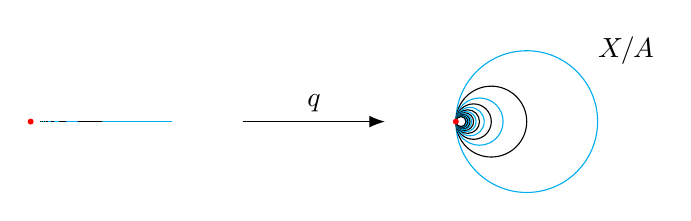
\begin{tikzpicture}[>={Latex[length=2mm]}, scale=1.8]
  \fill[red] (0,0) circle (0.6pt);
  \foreach \n in {1,...,14}{
    \pgfmathtruncatemacro{\p}{mod(\n,2)}
    \ifnum\p=1 \def\c{cyan}\else\def\c{black}\fi
    \draw[\c] ({1/\n},0)--({1/(\n+1)},0);
  }
  \draw[->] (1.5,0)--(2.5,0) node[midway,above] {$q$};
  \foreach \n in {1,...,14}{
    \pgfmathtruncatemacro{\p}{mod(\n,2)}
    \ifnum\p=1 \def\c{cyan}\else\def\c{black}\fi
    \draw[\c] ({3+1/(2*\n)},0) circle ({1/(2*\n)});
  }
  \fill[red] (3,0) circle (0.6pt);
  \node at (4.2,0.5) {$X/A$};
\end{tikzpicture}
\end{document}
